\documentclass[twoside]{book}

% Packages required by doxygen
\usepackage{fixltx2e}
\usepackage{calc}
\usepackage{doxygen}
\usepackage{graphicx}
\usepackage[utf8]{inputenc}
\usepackage{makeidx}
\usepackage{multicol}
\usepackage{multirow}
\PassOptionsToPackage{warn}{textcomp}
\usepackage{textcomp}
\usepackage[nointegrals]{wasysym}
\usepackage[table]{xcolor}

% Font selection
\usepackage[T1]{fontenc}
\usepackage{mathptmx}
\usepackage[scaled=.90]{helvet}
\usepackage{courier}
\usepackage{amssymb}
\usepackage{sectsty}
\renewcommand{\familydefault}{\sfdefault}
\allsectionsfont{%
  \fontseries{bc}\selectfont%
  \color{darkgray}%
}
\renewcommand{\DoxyLabelFont}{%
  \fontseries{bc}\selectfont%
  \color{darkgray}%
}
\newcommand{\+}{\discretionary{\mbox{\scriptsize$\hookleftarrow$}}{}{}}

% Page & text layout
\usepackage{geometry}
\geometry{%
  a4paper,%
  top=2.5cm,%
  bottom=2.5cm,%
  left=2.5cm,%
  right=2.5cm%
}
\tolerance=750
\hfuzz=15pt
\hbadness=750
\setlength{\emergencystretch}{15pt}
\setlength{\parindent}{0cm}
\setlength{\parskip}{0.2cm}
\makeatletter
\renewcommand{\paragraph}{%
  \@startsection{paragraph}{4}{0ex}{-1.0ex}{1.0ex}{%
    \normalfont\normalsize\bfseries\SS@parafont%
  }%
}
\renewcommand{\subparagraph}{%
  \@startsection{subparagraph}{5}{0ex}{-1.0ex}{1.0ex}{%
    \normalfont\normalsize\bfseries\SS@subparafont%
  }%
}
\makeatother

% Headers & footers
\usepackage{fancyhdr}
\pagestyle{fancyplain}
\fancyhead[LE]{\fancyplain{}{\bfseries\thepage}}
\fancyhead[CE]{\fancyplain{}{}}
\fancyhead[RE]{\fancyplain{}{\bfseries\leftmark}}
\fancyhead[LO]{\fancyplain{}{\bfseries\rightmark}}
\fancyhead[CO]{\fancyplain{}{}}
\fancyhead[RO]{\fancyplain{}{\bfseries\thepage}}
\fancyfoot[LE]{\fancyplain{}{}}
\fancyfoot[CE]{\fancyplain{}{}}
\fancyfoot[RE]{\fancyplain{}{\bfseries\scriptsize Generated on Sat Nov 8 2014 18\+:33\+:38 for My Project by Doxygen }}
\fancyfoot[LO]{\fancyplain{}{\bfseries\scriptsize Generated on Sat Nov 8 2014 18\+:33\+:38 for My Project by Doxygen }}
\fancyfoot[CO]{\fancyplain{}{}}
\fancyfoot[RO]{\fancyplain{}{}}
\renewcommand{\footrulewidth}{0.4pt}
\renewcommand{\chaptermark}[1]{%
  \markboth{#1}{}%
}
\renewcommand{\sectionmark}[1]{%
  \markright{\thesection\ #1}%
}

% Indices & bibliography
\usepackage{natbib}
\usepackage[titles]{tocloft}
\setcounter{tocdepth}{3}
\setcounter{secnumdepth}{5}
\makeindex

% Hyperlinks (required, but should be loaded last)
\usepackage{ifpdf}
\ifpdf
  \usepackage[pdftex,pagebackref=true]{hyperref}
\else
  \usepackage[ps2pdf,pagebackref=true]{hyperref}
\fi
\hypersetup{%
  colorlinks=true,%
  linkcolor=blue,%
  citecolor=blue,%
  unicode%
}

% Custom commands
\newcommand{\clearemptydoublepage}{%
  \newpage{\pagestyle{empty}\cleardoublepage}%
}


%===== C O N T E N T S =====

\begin{document}

% Titlepage & ToC
\hypersetup{pageanchor=false,
             bookmarks=true,
             bookmarksnumbered=true,
             pdfencoding=unicode
            }
\pagenumbering{roman}
\begin{titlepage}
\vspace*{7cm}
\begin{center}%
{\Large My Project }\\
\vspace*{1cm}
{\large Generated by Doxygen 1.8.8}\\
\vspace*{0.5cm}
{\small Sat Nov 8 2014 18:33:38}\\
\end{center}
\end{titlepage}
\clearemptydoublepage
\tableofcontents
\clearemptydoublepage
\pagenumbering{arabic}
\hypersetup{pageanchor=true}

%--- Begin generated contents ---
\chapter{Hierarchical Index}
\section{Class Hierarchy}
This inheritance list is sorted roughly, but not completely, alphabetically\+:\begin{DoxyCompactList}
\item \contentsline{section}{Bicicleta}{\pageref{class_bicicleta}}{}
\item \contentsline{section}{Data}{\pageref{class_data}}{}
\item \contentsline{section}{Empresa}{\pageref{class_empresa}}{}
\item \contentsline{section}{Posto\+Servico}{\pageref{class_posto_servico}}{}
\item \contentsline{section}{Rede}{\pageref{class_rede}}{}
\item \contentsline{section}{Registo}{\pageref{class_registo}}{}
\item \contentsline{section}{Utilizador}{\pageref{class_utilizador}}{}
\begin{DoxyCompactList}
\item \contentsline{section}{Ut\+\_\+ocasional}{\pageref{class_ut__ocasional}}{}
\end{DoxyCompactList}
\end{DoxyCompactList}

\chapter{Class Index}
\section{Class List}
Here are the classes, structs, unions and interfaces with brief descriptions\+:\begin{DoxyCompactList}
\item\contentsline{section}{\hyperlink{class_bicicleta}{Bicicleta} \\*\hyperlink{class_bicicleta}{Bicicleta} -\/ Auxiliary program class }{\pageref{class_bicicleta}}{}
\item\contentsline{section}{\hyperlink{class_data}{Data} \\*\hyperlink{class_data}{Data} -\/ auxiliary class to keep track of time }{\pageref{class_data}}{}
\item\contentsline{section}{\hyperlink{class_empresa}{Empresa} \\*\hyperlink{class_empresa}{Empresa} -\/ Auxiliary program class }{\pageref{class_empresa}}{}
\item\contentsline{section}{\hyperlink{class_posto_servico}{Posto\+Servico} \\*\hyperlink{class_posto_servico}{Posto\+Servico} -\/ Auxiliary program class }{\pageref{class_posto_servico}}{}
\item\contentsline{section}{\hyperlink{class_rede}{Rede} \\*\hyperlink{class_rede}{Rede} -\/ main program class }{\pageref{class_rede}}{}
\item\contentsline{section}{\hyperlink{class_registo}{Registo} \\*\hyperlink{class_registo}{Registo} -\/ Auxiliary program class }{\pageref{class_registo}}{}
\item\contentsline{section}{\hyperlink{class_ut__ocasional}{Ut\+\_\+ocasional} \\*\hyperlink{class_ut__ocasional}{Ut\+\_\+ocasional} -\/ occasional network users }{\pageref{class_ut__ocasional}}{}
\item\contentsline{section}{\hyperlink{class_utilizador}{Utilizador} \\*\hyperlink{class_utilizador}{Utilizador} -\/ class representing users of the network }{\pageref{class_utilizador}}{}
\end{DoxyCompactList}

\chapter{Class Documentation}
\hypertarget{class_bicicleta}{\section{Bicicleta Class Reference}
\label{class_bicicleta}\index{Bicicleta@{Bicicleta}}
}


\hyperlink{class_bicicleta}{Bicicleta} -\/ Auxiliary program class.  




{\ttfamily \#include $<$Bicicleta.\+h$>$}

\subsection*{Public Member Functions}
\begin{DoxyCompactItemize}
\item 
\hypertarget{class_bicicleta_af248a13124a9939cc3fa8eb3be56fdaf}{{\bfseries Bicicleta} (unsigned int id, string tipo\+\_\+bici, string size, int mudancas, bool avariad, unsigned int preco1)}\label{class_bicicleta_af248a13124a9939cc3fa8eb3be56fdaf}

\item 
\hypertarget{class_bicicleta_ac85afd4971d0b6eada6eb16f9a924118}{int {\bfseries get\+I\+D} ()}\label{class_bicicleta_ac85afd4971d0b6eada6eb16f9a924118}

\item 
\hypertarget{class_bicicleta_a956979f7f43934c329b143b9d6c2da49}{int {\bfseries get\+Velocidades} ()}\label{class_bicicleta_a956979f7f43934c329b143b9d6c2da49}

\item 
\hypertarget{class_bicicleta_a4582ea6f608f9d188df0b563961d7df5}{string {\bfseries get\+Tipo} ()}\label{class_bicicleta_a4582ea6f608f9d188df0b563961d7df5}

\item 
\hypertarget{class_bicicleta_a9733b1f60caff10aa814dfe38e8e459f}{string {\bfseries get\+Tamanho} ()}\label{class_bicicleta_a9733b1f60caff10aa814dfe38e8e459f}

\item 
\hypertarget{class_bicicleta_a98ab039cfa35975f6d1ff2223a625a7f}{string {\bfseries get\+Empresa} ()}\label{class_bicicleta_a98ab039cfa35975f6d1ff2223a625a7f}

\item 
\hypertarget{class_bicicleta_adcf9b86f83a83b15c98f70918469e664}{bool {\bfseries get\+Avariada} ()}\label{class_bicicleta_adcf9b86f83a83b15c98f70918469e664}

\item 
\hypertarget{class_bicicleta_a9e95e5a5744c9385a7a270876bf56f8c}{void {\bfseries set\+Avariada} ()}\label{class_bicicleta_a9e95e5a5744c9385a7a270876bf56f8c}

\item 
\hypertarget{class_bicicleta_adfccbf2a5c83a6c34c3454c78244cffc}{int {\bfseries get\+Preco} ()}\label{class_bicicleta_adfccbf2a5c83a6c34c3454c78244cffc}

\item 
\hypertarget{class_bicicleta_a830e5be0d74c904f9e1b4d0e46fcfbf6}{void {\bfseries set\+Preco\+Dia} (int velocidade, string tamanho)}\label{class_bicicleta_a830e5be0d74c904f9e1b4d0e46fcfbf6}

\item 
\hypertarget{class_bicicleta_a540f165785ed17b710a67c2a59991a48}{bool {\bfseries velocidades\+\_\+valido} (int veloc)}\label{class_bicicleta_a540f165785ed17b710a67c2a59991a48}

\item 
\hypertarget{class_bicicleta_a34990240a07a851793053ca4063a7b8e}{string {\bfseries tipo\+\_\+valido} ()}\label{class_bicicleta_a34990240a07a851793053ca4063a7b8e}

\item 
\hypertarget{class_bicicleta_a900359b6b195db211f479fe5929f8d81}{string {\bfseries imprime} ()}\label{class_bicicleta_a900359b6b195db211f479fe5929f8d81}

\item 
\hypertarget{class_bicicleta_a6e71bf61a37f13c3da8e620760f8f4b9}{void {\bfseries set\+I\+D} (int id)}\label{class_bicicleta_a6e71bf61a37f13c3da8e620760f8f4b9}

\item 
\hypertarget{class_bicicleta_a2318e7e7a22c44283e143f3c2942d721}{void {\bfseries set\+Tipo} (string tipo)}\label{class_bicicleta_a2318e7e7a22c44283e143f3c2942d721}

\item 
\hypertarget{class_bicicleta_ad5861007b46516987cab6fa7cf6adee1}{void {\bfseries set\+Regs\+Bicis} (vector$<$ \hyperlink{class_registo}{Registo} $\ast$ $>$ bicis)}\label{class_bicicleta_ad5861007b46516987cab6fa7cf6adee1}

\item 
\hypertarget{class_bicicleta_a05f9c922b7ebc82a1f223ba8c5d64cc2}{vector$<$ \hyperlink{class_registo}{Registo} $\ast$ $>$ {\bfseries get\+Regs\+Bicis} () const }\label{class_bicicleta_a05f9c922b7ebc82a1f223ba8c5d64cc2}

\item 
\hypertarget{class_bicicleta_a2520579ebcc40f9cc2ee05392f3004a2}{void {\bfseries adiciona\+Registo} (\hyperlink{class_registo}{Registo} $\ast$reg1)}\label{class_bicicleta_a2520579ebcc40f9cc2ee05392f3004a2}

\item 
\hypertarget{class_bicicleta_a28df135cc7d332d43ca85647fa60175a}{void {\bfseries set\+Tamanho} (string tamanho)}\label{class_bicicleta_a28df135cc7d332d43ca85647fa60175a}

\item 
\hypertarget{class_bicicleta_aef781f0496eab00a16c354d52f9f1686}{void {\bfseries set\+Veloc} (int velocidades)}\label{class_bicicleta_aef781f0496eab00a16c354d52f9f1686}

\item 
\hypertarget{class_bicicleta_a791cdbbf5016ea3a0229915b84a52a04}{bool {\bfseries remove\+\_\+util} (string nome)}\label{class_bicicleta_a791cdbbf5016ea3a0229915b84a52a04}

\item 
\hypertarget{class_bicicleta_a570101dbac9300d107433c52ae698915}{string {\bfseries get\+\_\+str} () const }\label{class_bicicleta_a570101dbac9300d107433c52ae698915}

\item 
\hypertarget{class_bicicleta_aff75cc7f6d1a554a8b7c663834115575}{void {\bfseries make\+\_\+str} (string bike)}\label{class_bicicleta_aff75cc7f6d1a554a8b7c663834115575}

\item 
void \hyperlink{class_bicicleta_ae48de57881e09ac89a84558c79894640}{set\+Empresa} (string emp)
\begin{DoxyCompactList}\small\item\em Sets the empresa attribute of the object to emp. \end{DoxyCompactList}\item 
\hypertarget{class_bicicleta_a0f6d8c8efea7822160a397ef040438d1}{\hyperlink{class_registo}{Registo} $\ast$ {\bfseries ultimo\+\_\+reg} () const }\label{class_bicicleta_a0f6d8c8efea7822160a397ef040438d1}

\end{DoxyCompactItemize}


\subsection{Detailed Description}
\hyperlink{class_bicicleta}{Bicicleta} -\/ Auxiliary program class. 

This class is used to represent bikes, storing all it's important features like size or type, identifying it with an I\+D and storing the record of it's use 

\subsection{Member Function Documentation}
\hypertarget{class_bicicleta_ae48de57881e09ac89a84558c79894640}{\index{Bicicleta@{Bicicleta}!set\+Empresa@{set\+Empresa}}
\index{set\+Empresa@{set\+Empresa}!Bicicleta@{Bicicleta}}
\subsubsection[{set\+Empresa}]{\setlength{\rightskip}{0pt plus 5cm}void Bicicleta\+::set\+Empresa (
\begin{DoxyParamCaption}
\item[{string}]{emp}
\end{DoxyParamCaption}
)\hspace{0.3cm}{\ttfamily [inline]}}}\label{class_bicicleta_ae48de57881e09ac89a84558c79894640}


Sets the empresa attribute of the object to emp. 


\begin{DoxyParams}{Parameters}
{\em emp} & -\/ New empresa for the object \\
\hline
\end{DoxyParams}


The documentation for this class was generated from the following files\+:\begin{DoxyCompactItemize}
\item 
\hyperlink{_bicicleta_8h}{Bicicleta.\+h}\item 
\hyperlink{_bicicleta_8cpp}{Bicicleta.\+cpp}\end{DoxyCompactItemize}

\hypertarget{class_data}{\section{Data Class Reference}
\label{class_data}\index{Data@{Data}}
}


\hyperlink{class_data}{Data} -\/ auxiliary class to keep track of time.  




{\ttfamily \#include $<$Data.\+h$>$}

\subsection*{Public Member Functions}
\begin{DoxyCompactItemize}
\item 
\hypertarget{class_data_af11f741cb7f587e2e495452a8905a22a}{\hyperlink{class_data_af11f741cb7f587e2e495452a8905a22a}{Data} ()}\label{class_data_af11f741cb7f587e2e495452a8905a22a}

\begin{DoxyCompactList}\small\item\em Default constructor of \hyperlink{class_data}{Data} class It initializes the object as being date 0000/00/00. \end{DoxyCompactList}\item 
\hyperlink{class_data_a2d45e272eb3ff0783c1603ddf7a44569}{Data} (unsigned int ano, unsigned int mes, unsigned int dia)
\begin{DoxyCompactList}\small\item\em Complete \hyperlink{class_data}{Data} constructor. \end{DoxyCompactList}\item 
\hyperlink{class_data_add8227267c76e3fecb385d7cd7fbcf4b}{Data} (string date)
\begin{DoxyCompactList}\small\item\em Constructor of Date from a string. \end{DoxyCompactList}\item 
string \hyperlink{class_data_a2a9f0b2202a6bf68215d3e06dc3cb57e}{get\+Data\+Str} () const 
\begin{DoxyCompactList}\small\item\em Convert \hyperlink{class_data}{Data} object to string This funtion converts the \hyperlink{class_data}{Data} object into a string in format Y\+Y\+Y\+Y/\+M\+M/\+D\+D. \end{DoxyCompactList}\end{DoxyCompactItemize}
\subsection*{Public Attributes}
\begin{DoxyCompactItemize}
\item 
\hypertarget{class_data_a1811fab972bdf6ed644c4eb7412bd043}{unsigned int {\bfseries ano}}\label{class_data_a1811fab972bdf6ed644c4eb7412bd043}

\item 
\hypertarget{class_data_a586deb479ec2031a0d3ceec8280f7706}{unsigned int {\bfseries mes}}\label{class_data_a586deb479ec2031a0d3ceec8280f7706}

\item 
\hypertarget{class_data_a71a904380d17858da0b902e9a2563546}{unsigned int {\bfseries dia}}\label{class_data_a71a904380d17858da0b902e9a2563546}

\end{DoxyCompactItemize}
\subsection*{Friends}
\begin{DoxyCompactItemize}
\item 
int \hyperlink{class_data_a950a6321928619d329831ee195416f79}{dif\+\_\+dias} (\hyperlink{class_data}{Data} d1, \hyperlink{class_data}{Data} d2)
\begin{DoxyCompactList}\small\item\em Calculates the difference between two dates in days. \end{DoxyCompactList}\item 
bool \hyperlink{class_data_a301f290080098e5d3983bdf4e870c3b9}{operator$<$} (const \hyperlink{class_data}{Data} data1, const \hyperlink{class_data}{Data} data2)
\begin{DoxyCompactList}\small\item\em Operator $<$ to compare \hyperlink{class_data}{Data} objects Compares two \hyperlink{class_data}{Data} objects to determine if one is \char`\"{}before\char`\"{} the other. \end{DoxyCompactList}\item 
bool \hyperlink{class_data_a3cf90128ca701a628213a73c2ae1d5ea}{operator==} (const \hyperlink{class_data}{Data} data1, const \hyperlink{class_data}{Data} data2)
\begin{DoxyCompactList}\small\item\em Operator == to determine equality of two \hyperlink{class_data}{Data} objects. \end{DoxyCompactList}\item 
ostream \& \hyperlink{class_data_a9daa61b4e0bee256d9481803c4778000}{operator$<$$<$} (ostream \&o, const \hyperlink{class_data}{Data} \&data)
\begin{DoxyCompactList}\small\item\em Allows operator $<$$<$ to use a \hyperlink{class_data}{Data} object Converts the object to a string using \hyperlink{class_data_a2a9f0b2202a6bf68215d3e06dc3cb57e}{get\+Data\+Str()} and \char`\"{}sends\char`\"{} it to the ostream o. \end{DoxyCompactList}\end{DoxyCompactItemize}


\subsection{Detailed Description}
\hyperlink{class_data}{Data} -\/ auxiliary class to keep track of time. 

This is a simple class we built to simplify the order of time in the rental events of \hyperlink{class_rede}{Rede}. Though, it was made in a way that it can be used in other, unrelated projects, because it has a simple, public, interface and has methods that allow easy convertion between \hyperlink{class_data}{Data} and other formats 

\subsection{Constructor \& Destructor Documentation}
\hypertarget{class_data_a2d45e272eb3ff0783c1603ddf7a44569}{\index{Data@{Data}!Data@{Data}}
\index{Data@{Data}!Data@{Data}}
\subsubsection[{Data}]{\setlength{\rightskip}{0pt plus 5cm}Data\+::\+Data (
\begin{DoxyParamCaption}
\item[{unsigned int}]{ano, }
\item[{unsigned int}]{mes, }
\item[{unsigned int}]{dia}
\end{DoxyParamCaption}
)}}\label{class_data_a2d45e272eb3ff0783c1603ddf7a44569}


Complete \hyperlink{class_data}{Data} constructor. 


\begin{DoxyParams}{Parameters}
{\em ano} & -\/ New object's year \\
\hline
{\em mes} & -\/ New object's month \\
\hline
{\em dia} & -\/ New object's day \\
\hline
\end{DoxyParams}
\hypertarget{class_data_add8227267c76e3fecb385d7cd7fbcf4b}{\index{Data@{Data}!Data@{Data}}
\index{Data@{Data}!Data@{Data}}
\subsubsection[{Data}]{\setlength{\rightskip}{0pt plus 5cm}Data\+::\+Data (
\begin{DoxyParamCaption}
\item[{string}]{date}
\end{DoxyParamCaption}
)}}\label{class_data_add8227267c76e3fecb385d7cd7fbcf4b}


Constructor of Date from a string. 


\begin{DoxyParams}{Parameters}
{\em date} & -\/ string with a date in format Y\+Y\+Y\+Y/\+M\+M/\+D\+D Constructs a date object from a string in the specified format, useful for construction of objects on load\+Info function of \hyperlink{class_rede}{Rede} class \\
\hline
\end{DoxyParams}


\subsection{Member Function Documentation}
\hypertarget{class_data_a2a9f0b2202a6bf68215d3e06dc3cb57e}{\index{Data@{Data}!get\+Data\+Str@{get\+Data\+Str}}
\index{get\+Data\+Str@{get\+Data\+Str}!Data@{Data}}
\subsubsection[{get\+Data\+Str}]{\setlength{\rightskip}{0pt plus 5cm}string Data\+::get\+Data\+Str (
\begin{DoxyParamCaption}
{}
\end{DoxyParamCaption}
) const}}\label{class_data_a2a9f0b2202a6bf68215d3e06dc3cb57e}


Convert \hyperlink{class_data}{Data} object to string This funtion converts the \hyperlink{class_data}{Data} object into a string in format Y\+Y\+Y\+Y/\+M\+M/\+D\+D. 

\begin{DoxyReturn}{Returns}
current \hyperlink{class_data}{Data} object in string format 
\end{DoxyReturn}


\subsection{Friends And Related Function Documentation}
\hypertarget{class_data_a950a6321928619d329831ee195416f79}{\index{Data@{Data}!dif\+\_\+dias@{dif\+\_\+dias}}
\index{dif\+\_\+dias@{dif\+\_\+dias}!Data@{Data}}
\subsubsection[{dif\+\_\+dias}]{\setlength{\rightskip}{0pt plus 5cm}int dif\+\_\+dias (
\begin{DoxyParamCaption}
\item[{{\bf Data}}]{d1, }
\item[{{\bf Data}}]{d2}
\end{DoxyParamCaption}
)\hspace{0.3cm}{\ttfamily [friend]}}}\label{class_data_a950a6321928619d329831ee195416f79}


Calculates the difference between two dates in days. 


\begin{DoxyParams}{Parameters}
{\em d1} & -\/ First \hyperlink{class_data}{Data} object \\
\hline
{\em d2} & -\/ Second \hyperlink{class_data}{Data} object \\
\hline
\end{DoxyParams}
\begin{DoxyReturn}{Returns}
day difference between two dates, given that d1 is \char`\"{}older\char`\"{} Calculates the difference between the two dates, considering the number of days in a month and other factors 
\end{DoxyReturn}
\hypertarget{class_data_a301f290080098e5d3983bdf4e870c3b9}{\index{Data@{Data}!operator$<$@{operator$<$}}
\index{operator$<$@{operator$<$}!Data@{Data}}
\subsubsection[{operator$<$}]{\setlength{\rightskip}{0pt plus 5cm}bool operator$<$ (
\begin{DoxyParamCaption}
\item[{const {\bf Data}}]{data1, }
\item[{const {\bf Data}}]{data2}
\end{DoxyParamCaption}
)\hspace{0.3cm}{\ttfamily [friend]}}}\label{class_data_a301f290080098e5d3983bdf4e870c3b9}


Operator $<$ to compare \hyperlink{class_data}{Data} objects Compares two \hyperlink{class_data}{Data} objects to determine if one is \char`\"{}before\char`\"{} the other. 


\begin{DoxyParams}{Parameters}
{\em data1} & -\/ First \hyperlink{class_data}{Data} object \\
\hline
{\em data2} & -\/ Second \hyperlink{class_data}{Data} object \\
\hline
\end{DoxyParams}
\begin{DoxyReturn}{Returns}
true if data1 is prior to data2, and false otherwise 
\end{DoxyReturn}
\hypertarget{class_data_a9daa61b4e0bee256d9481803c4778000}{\index{Data@{Data}!operator$<$$<$@{operator$<$$<$}}
\index{operator$<$$<$@{operator$<$$<$}!Data@{Data}}
\subsubsection[{operator$<$$<$}]{\setlength{\rightskip}{0pt plus 5cm}ostream\& operator$<$$<$ (
\begin{DoxyParamCaption}
\item[{ostream \&}]{o, }
\item[{const {\bf Data} \&}]{data}
\end{DoxyParamCaption}
)\hspace{0.3cm}{\ttfamily [friend]}}}\label{class_data_a9daa61b4e0bee256d9481803c4778000}


Allows operator $<$$<$ to use a \hyperlink{class_data}{Data} object Converts the object to a string using \hyperlink{class_data_a2a9f0b2202a6bf68215d3e06dc3cb57e}{get\+Data\+Str()} and \char`\"{}sends\char`\"{} it to the ostream o. 

\begin{DoxyReturn}{Returns}
ostream reference to allow multiple, inline, $<$$<$ operators 
\end{DoxyReturn}
\hypertarget{class_data_a3cf90128ca701a628213a73c2ae1d5ea}{\index{Data@{Data}!operator==@{operator==}}
\index{operator==@{operator==}!Data@{Data}}
\subsubsection[{operator==}]{\setlength{\rightskip}{0pt plus 5cm}bool operator== (
\begin{DoxyParamCaption}
\item[{const {\bf Data}}]{data1, }
\item[{const {\bf Data}}]{data2}
\end{DoxyParamCaption}
)\hspace{0.3cm}{\ttfamily [friend]}}}\label{class_data_a3cf90128ca701a628213a73c2ae1d5ea}


Operator == to determine equality of two \hyperlink{class_data}{Data} objects. 


\begin{DoxyParams}{Parameters}
{\em data1} & -\/ First \hyperlink{class_data}{Data} object \\
\hline
{\em data2} & -\/ Second \hyperlink{class_data}{Data} object \\
\hline
\end{DoxyParams}
\begin{DoxyReturn}{Returns}
true if data1 is equal to data2, and false otherwise 
\end{DoxyReturn}


The documentation for this class was generated from the following files\+:\begin{DoxyCompactItemize}
\item 
\hyperlink{_data_8h}{Data.\+h}\item 
\hyperlink{_data_8cpp}{Data.\+cpp}\end{DoxyCompactItemize}

\hypertarget{class_empresa}{\section{Empresa Class Reference}
\label{class_empresa}\index{Empresa@{Empresa}}
}
\subsection*{Public Member Functions}
\begin{DoxyCompactItemize}
\item 
\hypertarget{class_empresa_ac5bccaf3758b25fea4803a63d4362236}{{\bfseries Empresa} (string nome)}\label{class_empresa_ac5bccaf3758b25fea4803a63d4362236}

\item 
\hypertarget{class_empresa_a22e7cb6769eca729ad9f9d8a0cb0168a}{string {\bfseries get\+Nome} () const }\label{class_empresa_a22e7cb6769eca729ad9f9d8a0cb0168a}

\item 
\hypertarget{class_empresa_a0cd3335f43eb48e7da506a454d95fdb5}{int {\bfseries num\+\_\+users} () const }\label{class_empresa_a0cd3335f43eb48e7da506a454d95fdb5}

\item 
\hypertarget{class_empresa_aa5786b3765e8321ca420b0c5be4bb21c}{vector$<$ \hyperlink{class_bicicleta}{Bicicleta} $\ast$ $>$ {\bfseries get\+Bicicletas} () const }\label{class_empresa_aa5786b3765e8321ca420b0c5be4bb21c}

\item 
\hypertarget{class_empresa_a1b02af861954e1ddfd89c988faa62895}{void {\bfseries adiciona\+Bicicleta} (\hyperlink{class_bicicleta}{Bicicleta} $\ast$bic)}\label{class_empresa_a1b02af861954e1ddfd89c988faa62895}

\item 
\hypertarget{class_empresa_a585cffc1ecf217ea29827fb8e7fd6091}{void {\bfseries set\+Bicicletas} (const vector$<$ \hyperlink{class_bicicleta}{Bicicleta} $\ast$ $>$ bicicletas)}\label{class_empresa_a585cffc1ecf217ea29827fb8e7fd6091}

\item 
\hypertarget{class_empresa_ac09f08cdc3415311fd222cfadbaf6cb4}{void {\bfseries remove\+\_\+bicis} (unsigned int id)}\label{class_empresa_ac09f08cdc3415311fd222cfadbaf6cb4}

\item 
\hypertarget{class_empresa_aa7fb06c4029739ea9e33216942cb4686}{void {\bfseries show\+\_\+specs} ()}\label{class_empresa_aa7fb06c4029739ea9e33216942cb4686}

\item 
\hypertarget{class_empresa_a86f2b94b2ea2e7b11edbf645b4e55bac}{void {\bfseries set\+Nome} (string novo\+\_\+nome)}\label{class_empresa_a86f2b94b2ea2e7b11edbf645b4e55bac}

\end{DoxyCompactItemize}


The documentation for this class was generated from the following files\+:\begin{DoxyCompactItemize}
\item 
Empresa.\+h\item 
Empresa.\+cpp\end{DoxyCompactItemize}

\hypertarget{class_posto_servico}{\section{Posto\+Servico Class Reference}
\label{class_posto_servico}\index{Posto\+Servico@{Posto\+Servico}}
}
\subsection*{Public Member Functions}
\begin{DoxyCompactItemize}
\item 
\hypertarget{class_posto_servico_a53b6ddb92aebadb5168570cbf9f87bae}{{\bfseries Posto\+Servico} (int i\+D, int ocupacao, int lotacao)}\label{class_posto_servico_a53b6ddb92aebadb5168570cbf9f87bae}

\item 
\hypertarget{class_posto_servico_a12d2e1c64b373009aec51fb7f4df44ec}{int {\bfseries get\+I\+D} () const }\label{class_posto_servico_a12d2e1c64b373009aec51fb7f4df44ec}

\item 
\hypertarget{class_posto_servico_a467b1b77cd1a56131f0e5a6776a55885}{int {\bfseries get\+Lotacao} () const }\label{class_posto_servico_a467b1b77cd1a56131f0e5a6776a55885}

\item 
\hypertarget{class_posto_servico_a2f09c305c18b3c08686a852e2e8702ac}{int {\bfseries get\+Ocupacao} () const }\label{class_posto_servico_a2f09c305c18b3c08686a852e2e8702ac}

\item 
\hypertarget{class_posto_servico_a9efdef3b0af8965d366dacb6e61bb6d9}{int {\bfseries get\+Espaco\+Livre} () const }\label{class_posto_servico_a9efdef3b0af8965d366dacb6e61bb6d9}

\item 
\hypertarget{class_posto_servico_a0d3be8347bcfe2ff61915f0fe4688f11}{vector$<$ \hyperlink{class_bicicleta}{Bicicleta} $\ast$ $>$ {\bfseries get\+Disponiveis} ()}\label{class_posto_servico_a0d3be8347bcfe2ff61915f0fe4688f11}

\item 
\hypertarget{class_posto_servico_ae2675fbf3044cd0cc366fbec67449969}{vector$<$ \hyperlink{class_bicicleta}{Bicicleta} $\ast$ $>$ {\bfseries get\+Avariadas} ()}\label{class_posto_servico_ae2675fbf3044cd0cc366fbec67449969}

\item 
\hypertarget{class_posto_servico_a747fd34e7c83f28f1697284b6e139e2e}{vector$<$ \hyperlink{class_bicicleta}{Bicicleta} $\ast$ $>$ {\bfseries get\+Bicicletas} ()}\label{class_posto_servico_a747fd34e7c83f28f1697284b6e139e2e}

\item 
\hypertarget{class_posto_servico_abfe611099f0fb1d79f7a2344496af023}{vector$<$ \hyperlink{class_registo}{Registo} $\ast$ $>$ {\bfseries get\+Utlizacao} ()}\label{class_posto_servico_abfe611099f0fb1d79f7a2344496af023}

\item 
\hypertarget{class_posto_servico_afceba43d75e3b42c54cc6e8ff59ff22f}{void {\bfseries adicionabicicleta} (\hyperlink{class_bicicleta}{Bicicleta} $\ast$bi1)}\label{class_posto_servico_afceba43d75e3b42c54cc6e8ff59ff22f}

\item 
\hypertarget{class_posto_servico_a1b250081e0af407dc3ea0e7755da99a2}{void {\bfseries adiciona\+Disponivel} (\hyperlink{class_bicicleta}{Bicicleta} $\ast$bi1)}\label{class_posto_servico_a1b250081e0af407dc3ea0e7755da99a2}

\item 
\hypertarget{class_posto_servico_a2e01d6a12f30c50ca8c6d2eb50b33e0e}{void {\bfseries adiciona\+Avariada} (\hyperlink{class_bicicleta}{Bicicleta} $\ast$bi1)}\label{class_posto_servico_a2e01d6a12f30c50ca8c6d2eb50b33e0e}

\item 
\hypertarget{class_posto_servico_a0371ddda624f3760c76f04a4b6e767d0}{void {\bfseries adiciona\+Utilizacao} (\hyperlink{class_registo}{Registo} $\ast$reg1)}\label{class_posto_servico_a0371ddda624f3760c76f04a4b6e767d0}

\item 
\hypertarget{class_posto_servico_a0ee0fe238467db3ea6f207d528a6e2e9}{void {\bfseries set\+Disponiveis} (vector$<$ \hyperlink{class_bicicleta}{Bicicleta} $\ast$ $>$ disponiveis)}\label{class_posto_servico_a0ee0fe238467db3ea6f207d528a6e2e9}

\item 
\hypertarget{class_posto_servico_afb5c121f880c880bdcc75033eb9bc7f2}{void {\bfseries set\+Avariadas} (vector$<$ \hyperlink{class_bicicleta}{Bicicleta} $\ast$ $>$ avariadas)}\label{class_posto_servico_afb5c121f880c880bdcc75033eb9bc7f2}

\item 
\hypertarget{class_posto_servico_ae63f7836c55f4eb38d8916c140f62162}{void {\bfseries set\+Utilizacao} (vector$<$ \hyperlink{class_registo}{Registo} $\ast$ $>$ utilizacao)}\label{class_posto_servico_ae63f7836c55f4eb38d8916c140f62162}

\item 
\hypertarget{class_posto_servico_a68ca412e4456c344981f6cb0b01c4184}{void {\bfseries set\+I\+D} (int id)}\label{class_posto_servico_a68ca412e4456c344981f6cb0b01c4184}

\item 
\hypertarget{class_posto_servico_a0acde19dbfc74b355e1aa2e34f25fa11}{void {\bfseries set\+Lotacao} (int lot)}\label{class_posto_servico_a0acde19dbfc74b355e1aa2e34f25fa11}

\item 
\hypertarget{class_posto_servico_a30d51d2560c0239ecb513db121a604a7}{bool {\bfseries aluga} (\hyperlink{class_bicicleta}{Bicicleta} $\ast$bi1)}\label{class_posto_servico_a30d51d2560c0239ecb513db121a604a7}

\item 
\hypertarget{class_posto_servico_a9b7c97136f4b1e2cc7d90cbdb54c3f53}{bool {\bfseries devolve} (\hyperlink{class_bicicleta}{Bicicleta} $\ast$bi1)}\label{class_posto_servico_a9b7c97136f4b1e2cc7d90cbdb54c3f53}

\item 
\hypertarget{class_posto_servico_a01c59324f65bf70ce5400718cde0791a}{bool {\bfseries removebicicleta} (unsigned int id\+\_\+bike)}\label{class_posto_servico_a01c59324f65bf70ce5400718cde0791a}

\item 
\hypertarget{class_posto_servico_a9cab807cf7fcecad5e8231abdb7ef491}{bool {\bfseries removeutilizador} (string user)}\label{class_posto_servico_a9cab807cf7fcecad5e8231abdb7ef491}

\item 
\hypertarget{class_posto_servico_a15a1ac03805060f0b2282e32c8f95da2}{void {\bfseries arranja\+\_\+bicicletas} ()}\label{class_posto_servico_a15a1ac03805060f0b2282e32c8f95da2}

\item 
\hypertarget{class_posto_servico_a116efc301c6955001083ba199ed96ed2}{bool {\bfseries arranja\+\_\+bicicleta} (int id\+\_\+bike)}\label{class_posto_servico_a116efc301c6955001083ba199ed96ed2}

\end{DoxyCompactItemize}


The documentation for this class was generated from the following files\+:\begin{DoxyCompactItemize}
\item 
Posto\+Servico.\+h\item 
Posto\+Servico.\+cpp\end{DoxyCompactItemize}

\hypertarget{class_rede}{\section{Rede Class Reference}
\label{class_rede}\index{Rede@{Rede}}
}
\subsection*{Public Member Functions}
\begin{DoxyCompactItemize}
\item 
\hypertarget{class_rede_a1751f922073f6172ba676a56959a1540}{void {\bfseries load\+Info} ()}\label{class_rede_a1751f922073f6172ba676a56959a1540}

\item 
\hypertarget{class_rede_abec1da6660663cd58e6851737219959e}{void {\bfseries store\+Info} ()}\label{class_rede_abec1da6660663cd58e6851737219959e}

\item 
\hypertarget{class_rede_ae78851a9d7efe2a9e0d2ead64f68ef73}{int {\bfseries add\+User} (\hyperlink{class_utilizador}{Utilizador} user)}\label{class_rede_ae78851a9d7efe2a9e0d2ead64f68ef73}

\item 
\hypertarget{class_rede_a39d746dc37d11b8c870701a3afa9328e}{int {\bfseries create\+User} (string nome)}\label{class_rede_a39d746dc37d11b8c870701a3afa9328e}

\item 
\hypertarget{class_rede_a00b09749f19ec7535127e75531281511}{void {\bfseries add\+Posto} (\hyperlink{class_posto_servico}{Posto\+Servico} $\ast$posto)}\label{class_rede_a00b09749f19ec7535127e75531281511}

\item 
\hypertarget{class_rede_a4177da39d4aa05cd0451d52a7220b7c5}{int {\bfseries create\+\_\+add\+\_\+bike} ()}\label{class_rede_a4177da39d4aa05cd0451d52a7220b7c5}

\item 
\hypertarget{class_rede_adec8c4515163174c0fab8068e36c6cc5}{void {\bfseries reset} ()}\label{class_rede_adec8c4515163174c0fab8068e36c6cc5}

\item 
\hypertarget{class_rede_ad38e26e59622727f978b995f6b9955c5}{void {\bfseries assign\+\_\+regs} (vector$<$ \hyperlink{class_registo}{Registo} $\ast$ $>$ \&regs)}\label{class_rede_ad38e26e59622727f978b995f6b9955c5}

\item 
\hypertarget{class_rede_a42b5a88380e63b78e5c99894aee0dfbc}{bool {\bfseries existe\+Utilizador} (string nome)}\label{class_rede_a42b5a88380e63b78e5c99894aee0dfbc}

\item 
\hypertarget{class_rede_ac74ae338ed2ddb5b8f94c9ed33e172ef}{int {\bfseries tipo\+User} (string nome)}\label{class_rede_ac74ae338ed2ddb5b8f94c9ed33e172ef}

\item 
\hypertarget{class_rede_aba033af0c2cd9a4f70ca1f9459a6a3ee}{string {\bfseries is\+\_\+busy} (int id\+\_\+bici, bool print) const }\label{class_rede_aba033af0c2cd9a4f70ca1f9459a6a3ee}

\item 
\hypertarget{class_rede_a0862364a4ce27c157b2b756184526748}{vector$<$ \hyperlink{class_registo}{Registo} $\ast$ $>$ {\bfseries get\+\_\+regs} () const }\label{class_rede_a0862364a4ce27c157b2b756184526748}

\item 
\hypertarget{class_rede_a906023ec85b2043b4610e627951e93b8}{int {\bfseries menu\+\_\+system} ()}\label{class_rede_a906023ec85b2043b4610e627951e93b8}

\item 
\hypertarget{class_rede_a7f6b41951357f14d8be5c0c23f59bca9}{void {\bfseries print\+\_\+menu\+\_\+header} ()}\label{class_rede_a7f6b41951357f14d8be5c0c23f59bca9}

\item 
\hypertarget{class_rede_ab94437bdbb3cb32b8489591748c1a57e}{void {\bfseries menu\+\_\+exit\+\_\+prog} ()}\label{class_rede_ab94437bdbb3cb32b8489591748c1a57e}

\item 
\hypertarget{class_rede_ad5f01d997329c28cc736b42e9962c2b6}{int {\bfseries menu\+\_\+start} ()}\label{class_rede_ad5f01d997329c28cc736b42e9962c2b6}

\item 
\hypertarget{class_rede_aa36d94723cae863269eb20375c4491c4}{int {\bfseries menu\+\_\+reg\+Usr} ()}\label{class_rede_aa36d94723cae863269eb20375c4491c4}

\item 
\hypertarget{class_rede_a8865f7a80236b7a399e948a486c86bac}{int {\bfseries menu\+\_\+oc\+Usr} ()}\label{class_rede_a8865f7a80236b7a399e948a486c86bac}

\item 
\hypertarget{class_rede_a71b157db8d1ec17c2e5100faeb95e3d2}{int {\bfseries menu\+\_\+manager} ()}\label{class_rede_a71b157db8d1ec17c2e5100faeb95e3d2}

\item 
\hypertarget{class_rede_af5dd3d55b3cb2f252349128787a96e27}{int {\bfseries menu\+\_\+reg\+Usr\+\_\+logged} (\hyperlink{class_utilizador}{Utilizador} $\ast$user)}\label{class_rede_af5dd3d55b3cb2f252349128787a96e27}

\item 
\hypertarget{class_rede_a11e8c9a0d004251882872f9cc3da54da}{int {\bfseries menu\+\_\+mngr\+\_\+supplyers} ()}\label{class_rede_a11e8c9a0d004251882872f9cc3da54da}

\item 
\hypertarget{class_rede_a0d7d6e769f20ff9f3ce54441ec88727e}{int {\bfseries menu\+\_\+mngr\+\_\+spots} ()}\label{class_rede_a0d7d6e769f20ff9f3ce54441ec88727e}

\item 
\hypertarget{class_rede_a2f83a9dde6e018ac57f1aefcfca388b2}{int {\bfseries menu\+\_\+mngr\+\_\+bikes} ()}\label{class_rede_a2f83a9dde6e018ac57f1aefcfca388b2}

\item 
\hypertarget{class_rede_a609866278eb7f37d19397f078a5a6ea6}{int {\bfseries menu\+\_\+mngr\+\_\+users} ()}\label{class_rede_a609866278eb7f37d19397f078a5a6ea6}

\item 
\hypertarget{class_rede_ae11dd331c071a1d4dace9fc89d82e251}{int {\bfseries menu\+\_\+mngr\+\_\+logs} ()}\label{class_rede_ae11dd331c071a1d4dace9fc89d82e251}

\end{DoxyCompactItemize}


The documentation for this class was generated from the following files\+:\begin{DoxyCompactItemize}
\item 
Rede.\+h\item 
Rede.\+cpp\end{DoxyCompactItemize}

\hypertarget{class_registo}{\section{Registo Class Reference}
\label{class_registo}\index{Registo@{Registo}}
}
\subsection*{Public Member Functions}
\begin{DoxyCompactItemize}
\item 
\hypertarget{class_registo_a17d5d8a67903e30624817b5798c6065e}{void {\bfseries print\+\_\+reg} () const }\label{class_registo_a17d5d8a67903e30624817b5798c6065e}

\item 
\hypertarget{class_registo_a80d93fbe1e4ea760aea6e3cf74a8bcce}{void {\bfseries print\+\_\+sem\+\_\+user} () const }\label{class_registo_a80d93fbe1e4ea760aea6e3cf74a8bcce}

\item 
\hypertarget{class_registo_ad0220e2d516af222c01893634eace4d4}{string {\bfseries get\+\_\+str} () const }\label{class_registo_ad0220e2d516af222c01893634eace4d4}

\item 
\hypertarget{class_registo_aa377d8fc39a2efda5ae6452f618635c2}{void {\bfseries make\+\_\+from\+\_\+str} (string reg)}\label{class_registo_aa377d8fc39a2efda5ae6452f618635c2}

\end{DoxyCompactItemize}
\subsection*{Public Attributes}
\begin{DoxyCompactItemize}
\item 
\hypertarget{class_registo_af745f6be9e0f119ff8285f2ad7bc0007}{int {\bfseries I\+D\+\_\+\+Bicicleta}}\label{class_registo_af745f6be9e0f119ff8285f2ad7bc0007}

\item 
\hypertarget{class_registo_ab1eceed0788883d77f331da0eed92876}{int {\bfseries I\+D\+\_\+posto\+\_\+origem}}\label{class_registo_ab1eceed0788883d77f331da0eed92876}

\item 
\hypertarget{class_registo_a95a2f4c5bbad742f0ccdfc0da873a2c2}{int {\bfseries I\+D\+\_\+posto\+\_\+chegada}}\label{class_registo_a95a2f4c5bbad742f0ccdfc0da873a2c2}

\item 
\hypertarget{class_registo_a58143db2825d4cc53f502001fa5d7659}{string {\bfseries nome\+\_\+utilizador}}\label{class_registo_a58143db2825d4cc53f502001fa5d7659}

\item 
\hypertarget{class_registo_ac0d3e2faff6e42050b6f75a3db8ae92b}{\hyperlink{class_data}{Data} {\bfseries levantamento}}\label{class_registo_ac0d3e2faff6e42050b6f75a3db8ae92b}

\item 
\hypertarget{class_registo_a051ce058418ededccbe9aae6900cd817}{\hyperlink{class_data}{Data} {\bfseries entrega}}\label{class_registo_a051ce058418ededccbe9aae6900cd817}

\item 
\hypertarget{class_registo_afa35faa61b95b63bbab972cfaca38b98}{bool {\bfseries ficou\+\_\+avariada}}\label{class_registo_afa35faa61b95b63bbab972cfaca38b98}

\end{DoxyCompactItemize}
\subsection*{Friends}
\begin{DoxyCompactItemize}
\item 
\hypertarget{class_registo_aaf8e089b26abe6bc63d1c2399433bce6}{bool {\bfseries operator==} (const \hyperlink{class_registo}{Registo} reg1, const \hyperlink{class_registo}{Registo} reg2)}\label{class_registo_aaf8e089b26abe6bc63d1c2399433bce6}

\end{DoxyCompactItemize}


The documentation for this class was generated from the following files\+:\begin{DoxyCompactItemize}
\item 
Registo.\+h\item 
Registo.\+cpp\end{DoxyCompactItemize}

\hypertarget{class_ut__ocasional}{\section{Ut\+\_\+ocasional Class Reference}
\label{class_ut__ocasional}\index{Ut\+\_\+ocasional@{Ut\+\_\+ocasional}}
}


\hyperlink{class_ut__ocasional}{Ut\+\_\+ocasional} -\/ occasional network users.  




{\ttfamily \#include $<$Utilizador.\+h$>$}

Inheritance diagram for Ut\+\_\+ocasional\+:\begin{figure}[H]
\begin{center}
\leavevmode
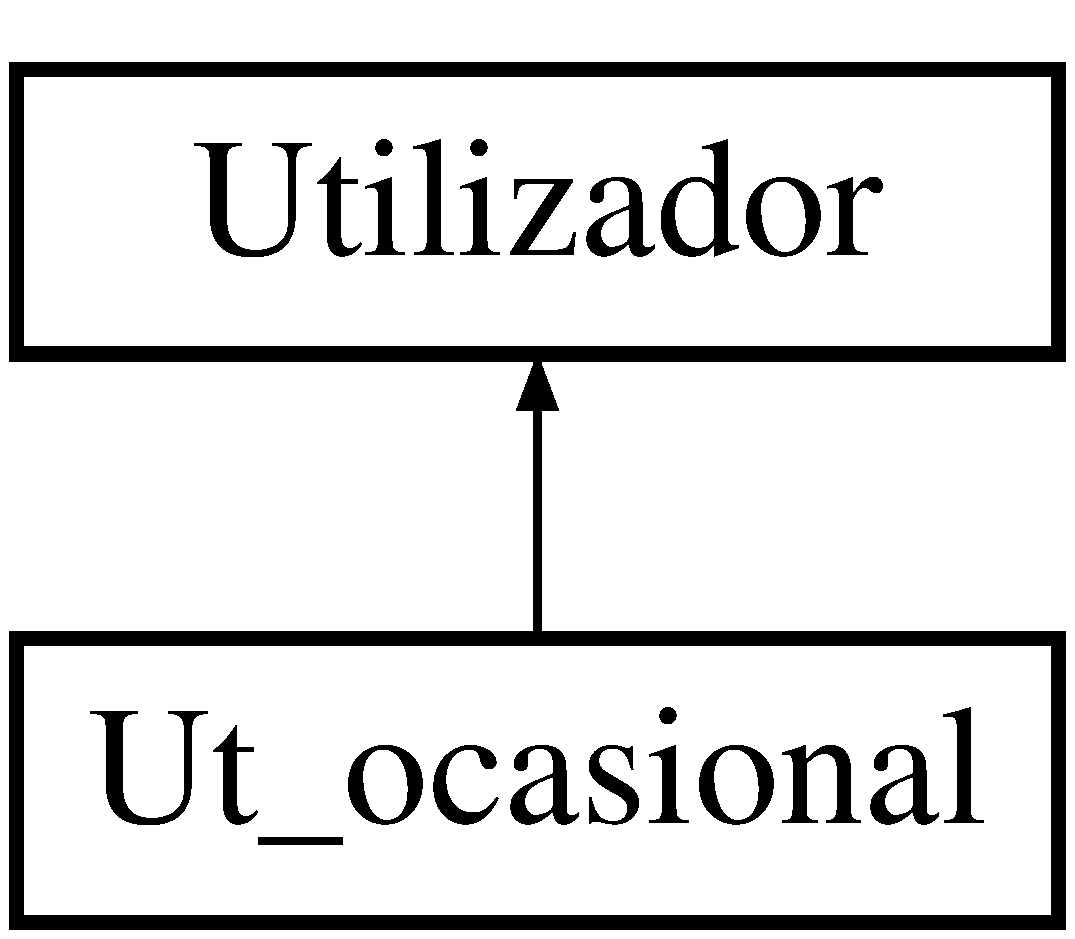
\includegraphics[height=2.000000cm]{class_ut__ocasional}
\end{center}
\end{figure}
\subsection*{Public Member Functions}
\begin{DoxyCompactItemize}
\item 
\hypertarget{class_ut__ocasional_ad26b95c8f79ed12f221da29f19896e82}{\hyperlink{class_ut__ocasional_ad26b95c8f79ed12f221da29f19896e82}{Ut\+\_\+ocasional} ()}\label{class_ut__ocasional_ad26b95c8f79ed12f221da29f19896e82}

\begin{DoxyCompactList}\small\item\em Default constructor of \hyperlink{class_ut__ocasional}{Ut\+\_\+ocasional} Initializes everything like \hyperlink{class_utilizador}{Utilizador} default constructor, except for tipo (now equal to 1) \end{DoxyCompactList}\item 
\hypertarget{class_ut__ocasional_acf3a4c7d6ef3d9000c6284a93201d4b1}{\hyperlink{class_ut__ocasional_acf3a4c7d6ef3d9000c6284a93201d4b1}{Ut\+\_\+ocasional} (string name, int age, string pass, string novo\+\_\+cartao)}\label{class_ut__ocasional_acf3a4c7d6ef3d9000c6284a93201d4b1}

\begin{DoxyCompactList}\small\item\em Complete constructor of \hyperlink{class_ut__ocasional}{Ut\+\_\+ocasional}. \end{DoxyCompactList}\item 
\hypertarget{class_ut__ocasional_a5a455dacffda809dd8a383896174dd07}{string {\bfseries get\+\_\+cartao} ()}\label{class_ut__ocasional_a5a455dacffda809dd8a383896174dd07}

\item 
\hypertarget{class_ut__ocasional_a4c4005d41c818c737d56121ec9a79e19}{void {\bfseries set\+\_\+cartao} (string novo)}\label{class_ut__ocasional_a4c4005d41c818c737d56121ec9a79e19}

\item 
int \hyperlink{class_ut__ocasional_a372c795cc67b402e54dc78e6e24c3779}{get\+Custo} ()
\begin{DoxyCompactList}\small\item\em Get service cost for \hyperlink{class_ut__ocasional}{Ut\+\_\+ocasional} Redefinition of the same funtion on \hyperlink{class_utilizador}{Utilizador} class. \end{DoxyCompactList}\item 
string \hyperlink{class_ut__ocasional_a500c4745815fed11a495c258a06f973a}{get\+\_\+str} () const 
\begin{DoxyCompactList}\small\item\em Get string that represents user This function is used in \hyperlink{class_rede_abec1da6660663cd58e6851737219959e}{Rede\+::store\+Info()}, because it converts the \hyperlink{class_ut__ocasional}{Ut\+\_\+ocasional} object to a multiple line string containing all of it's information except the rental logs. \end{DoxyCompactList}\item 
\hypertarget{class_ut__ocasional_a215c8d086f1285c12e5bb8b42ccef682}{void \hyperlink{class_ut__ocasional_a215c8d086f1285c12e5bb8b42ccef682}{make\+\_\+str} (string user)}\label{class_ut__ocasional_a215c8d086f1285c12e5bb8b42ccef682}

\begin{DoxyCompactList}\small\item\em Make a user from a string that represents it (in this case, a \hyperlink{class_ut__ocasional}{Ut\+\_\+ocasional} user) This function is used in \hyperlink{class_rede_a1751f922073f6172ba676a56959a1540}{Rede\+::load\+Info()}, because it makes a \hyperlink{class_ut__ocasional}{Ut\+\_\+ocasional} object from a multiple line string that contains all it's information except for the rental logs. \end{DoxyCompactList}\end{DoxyCompactItemize}
\subsection*{Additional Inherited Members}


\subsection{Detailed Description}
\hyperlink{class_ut__ocasional}{Ut\+\_\+ocasional} -\/ occasional network users. 

This class stores information for occasional users. It is derived of \hyperlink{class_utilizador}{Utilizador}, because it only adds the user's credit card. Since, for this type of user, age and password are irrelevant, it initializes password as an empty string and age as 5 

\subsection{Member Function Documentation}
\hypertarget{class_ut__ocasional_a500c4745815fed11a495c258a06f973a}{\index{Ut\+\_\+ocasional@{Ut\+\_\+ocasional}!get\+\_\+str@{get\+\_\+str}}
\index{get\+\_\+str@{get\+\_\+str}!Ut\+\_\+ocasional@{Ut\+\_\+ocasional}}
\subsubsection[{get\+\_\+str}]{\setlength{\rightskip}{0pt plus 5cm}string Ut\+\_\+ocasional\+::get\+\_\+str (
\begin{DoxyParamCaption}
{}
\end{DoxyParamCaption}
) const\hspace{0.3cm}{\ttfamily [virtual]}}}\label{class_ut__ocasional_a500c4745815fed11a495c258a06f973a}


Get string that represents user This function is used in \hyperlink{class_rede_abec1da6660663cd58e6851737219959e}{Rede\+::store\+Info()}, because it converts the \hyperlink{class_ut__ocasional}{Ut\+\_\+ocasional} object to a multiple line string containing all of it's information except the rental logs. 

\begin{DoxyReturn}{Returns}
string representing user info 
\end{DoxyReturn}


Reimplemented from \hyperlink{class_utilizador_a79a6281b24b8ecf31b25e41f5650843d}{Utilizador}.

\hypertarget{class_ut__ocasional_a372c795cc67b402e54dc78e6e24c3779}{\index{Ut\+\_\+ocasional@{Ut\+\_\+ocasional}!get\+Custo@{get\+Custo}}
\index{get\+Custo@{get\+Custo}!Ut\+\_\+ocasional@{Ut\+\_\+ocasional}}
\subsubsection[{get\+Custo}]{\setlength{\rightskip}{0pt plus 5cm}int Ut\+\_\+ocasional\+::get\+Custo (
\begin{DoxyParamCaption}
{}
\end{DoxyParamCaption}
)\hspace{0.3cm}{\ttfamily [virtual]}}}\label{class_ut__ocasional_a372c795cc67b402e54dc78e6e24c3779}


Get service cost for \hyperlink{class_ut__ocasional}{Ut\+\_\+ocasional} Redefinition of the same funtion on \hyperlink{class_utilizador}{Utilizador} class. 

\begin{DoxyReturn}{Returns}
service cost for the \hyperlink{class_ut__ocasional}{Ut\+\_\+ocasional} user 
\end{DoxyReturn}


Reimplemented from \hyperlink{class_utilizador_a988e8a7c0cc0625866350a476a5d7b62}{Utilizador}.



The documentation for this class was generated from the following files\+:\begin{DoxyCompactItemize}
\item 
\hyperlink{_utilizador_8h}{Utilizador.\+h}\item 
\hyperlink{_utilizador_8cpp}{Utilizador.\+cpp}\end{DoxyCompactItemize}

\hypertarget{class_utilizador}{\section{Utilizador Class Reference}
\label{class_utilizador}\index{Utilizador@{Utilizador}}
}
Inheritance diagram for Utilizador\+:\begin{figure}[H]
\begin{center}
\leavevmode
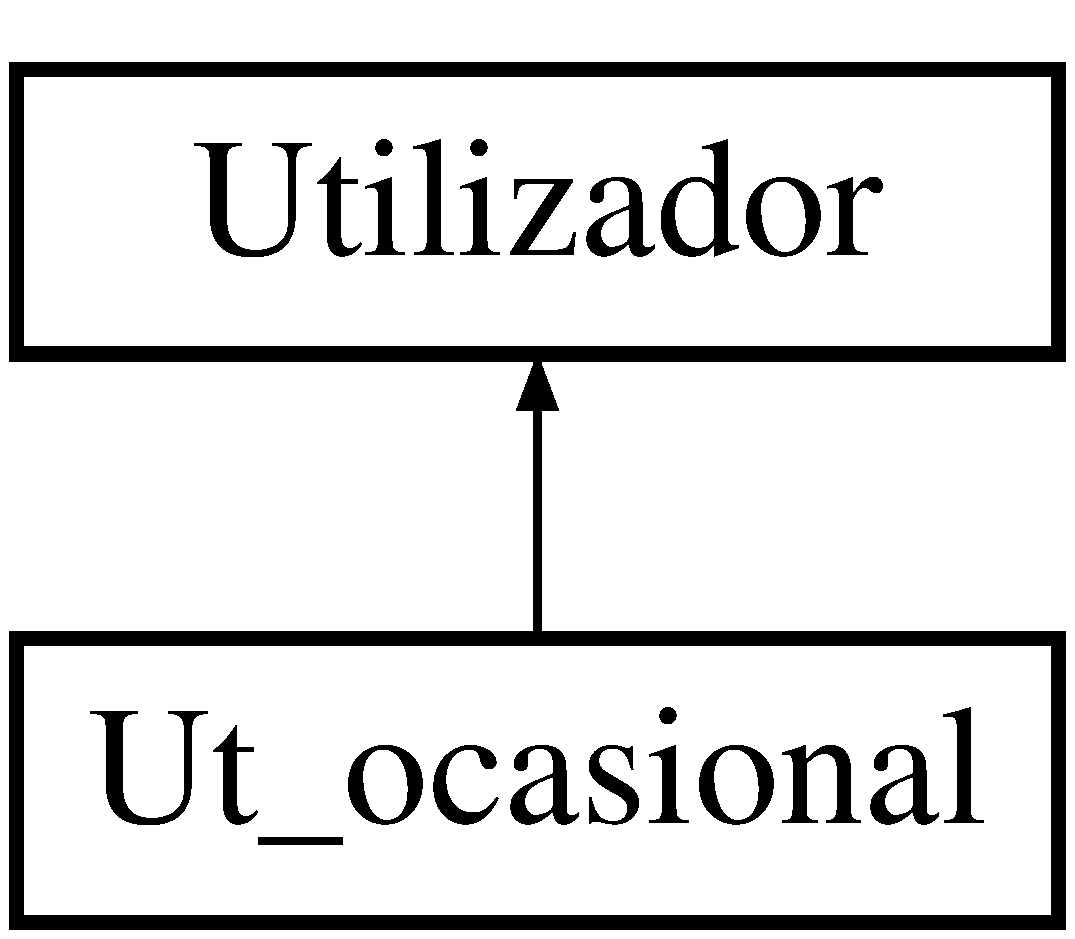
\includegraphics[height=2.000000cm]{class_utilizador}
\end{center}
\end{figure}
\subsection*{Public Member Functions}
\begin{DoxyCompactItemize}
\item 
\hypertarget{class_utilizador_a4ce0d50c55e4f03e61ffa97376a2f30c}{{\bfseries Utilizador} (string name, int age)}\label{class_utilizador_a4ce0d50c55e4f03e61ffa97376a2f30c}

\item 
\hypertarget{class_utilizador_a8764eb80a3f0f8c352628272f62dbd6d}{{\bfseries Utilizador} (string name, int age, string pass)}\label{class_utilizador_a8764eb80a3f0f8c352628272f62dbd6d}

\item 
\hypertarget{class_utilizador_a24f10fc3cfa2deb7aa38cc280722327a}{void {\bfseries set\+Nome} (string nome)}\label{class_utilizador_a24f10fc3cfa2deb7aa38cc280722327a}

\item 
\hypertarget{class_utilizador_a1201b047034f08dd8b1e8d4df36ca97b}{void {\bfseries set\+Idade} (int idade)}\label{class_utilizador_a1201b047034f08dd8b1e8d4df36ca97b}

\item 
\hypertarget{class_utilizador_aa5af9c1385b0a93116dd8a80264b887a}{string {\bfseries get\+Nome} () const }\label{class_utilizador_aa5af9c1385b0a93116dd8a80264b887a}

\item 
\hypertarget{class_utilizador_a9abaeb6fbff49683f57164a57e6f0c90}{int {\bfseries get\+Idade} () const }\label{class_utilizador_a9abaeb6fbff49683f57164a57e6f0c90}

\item 
\hypertarget{class_utilizador_a41730715f6cdd5bd98e3647150836989}{vector$<$ \hyperlink{class_registo}{Registo} $\ast$ $>$ {\bfseries get\+Regs} () const }\label{class_utilizador_a41730715f6cdd5bd98e3647150836989}

\item 
\hypertarget{class_utilizador_a6a319b5af1400354e5fc22056fbfefc5}{void {\bfseries set\+Regs} (vector$<$ \hyperlink{class_registo}{Registo} $\ast$ $>$ regs)}\label{class_utilizador_a6a319b5af1400354e5fc22056fbfefc5}

\item 
\hypertarget{class_utilizador_aadf5270d1131da77040b628c23ef89b2}{\hyperlink{class_registo}{Registo} $\ast$ {\bfseries ultimo\+Reg} () const }\label{class_utilizador_aadf5270d1131da77040b628c23ef89b2}

\item 
\hypertarget{class_utilizador_a8be0d01c3f23383c25596bd1c73918e4}{string {\bfseries get\+Password} () const }\label{class_utilizador_a8be0d01c3f23383c25596bd1c73918e4}

\item 
\hypertarget{class_utilizador_a14ffc9d7128ed6c99e7adc4f94315f56}{void {\bfseries set\+Password} (string pass)}\label{class_utilizador_a14ffc9d7128ed6c99e7adc4f94315f56}

\item 
\hypertarget{class_utilizador_a8d0083b685ee8023dd9bbf5b0372cb1d}{bool {\bfseries operator==} (string name)}\label{class_utilizador_a8d0083b685ee8023dd9bbf5b0372cb1d}

\item 
\hypertarget{class_utilizador_a668e5c9fd643f4e56dbdb2a6e1172bf5}{bool {\bfseries operator==} (\hyperlink{class_utilizador}{Utilizador} user)}\label{class_utilizador_a668e5c9fd643f4e56dbdb2a6e1172bf5}

\item 
\hypertarget{class_utilizador_a0ceb8bbbe6766b2f83ed9130fbf0975f}{void {\bfseries operator=} (\hyperlink{class_utilizador}{Utilizador} user)}\label{class_utilizador_a0ceb8bbbe6766b2f83ed9130fbf0975f}

\item 
\hypertarget{class_utilizador_a6282ddeeb794835afa4ce109ebb6b53a}{int {\bfseries get\+Tipo} ()}\label{class_utilizador_a6282ddeeb794835afa4ce109ebb6b53a}

\item 
\hypertarget{class_utilizador_a988e8a7c0cc0625866350a476a5d7b62}{virtual int {\bfseries get\+Custo} ()}\label{class_utilizador_a988e8a7c0cc0625866350a476a5d7b62}

\item 
\hypertarget{class_utilizador_a388ed972e4a98a3e09aca8edb9ad71a3}{void {\bfseries adiciona\+Registo} (\hyperlink{class_registo}{Registo} $\ast$reg)}\label{class_utilizador_a388ed972e4a98a3e09aca8edb9ad71a3}

\item 
\hypertarget{class_utilizador_a72e81f30a09f65dc12ad4388a1bb4c6f}{int {\bfseries tempo\+\_\+aluguer} ()}\label{class_utilizador_a72e81f30a09f65dc12ad4388a1bb4c6f}

\item 
\hypertarget{class_utilizador_a19b8e1ca2d9b0036e041bb9d1813b1be}{int {\bfseries num\+\_\+aluguer} ()}\label{class_utilizador_a19b8e1ca2d9b0036e041bb9d1813b1be}

\item 
\hypertarget{class_utilizador_aaad55e54d2ab5a5a8dbe0c98092ab77a}{void {\bfseries remove\+\_\+bici} (int id)}\label{class_utilizador_aaad55e54d2ab5a5a8dbe0c98092ab77a}

\item 
\hypertarget{class_utilizador_a79a6281b24b8ecf31b25e41f5650843d}{virtual string {\bfseries get\+\_\+str} () const }\label{class_utilizador_a79a6281b24b8ecf31b25e41f5650843d}

\item 
\hypertarget{class_utilizador_ae2d157ed39a4f4d8e96c288ac7de320d}{virtual void {\bfseries make\+\_\+str} (string user)}\label{class_utilizador_ae2d157ed39a4f4d8e96c288ac7de320d}

\end{DoxyCompactItemize}
\subsection*{Protected Attributes}
\begin{DoxyCompactItemize}
\item 
\hypertarget{class_utilizador_a3d22333263aef7b7a61a96b46ba7828d}{string {\bfseries nome}}\label{class_utilizador_a3d22333263aef7b7a61a96b46ba7828d}

\item 
\hypertarget{class_utilizador_aae4c416534c9b645e933cea05db50050}{string {\bfseries password}}\label{class_utilizador_aae4c416534c9b645e933cea05db50050}

\item 
\hypertarget{class_utilizador_aa4c6a81b2b5bb75690e9fb3c8d8412b6}{unsigned int {\bfseries idade}}\label{class_utilizador_aa4c6a81b2b5bb75690e9fb3c8d8412b6}

\item 
\hypertarget{class_utilizador_a2b89c422324741fe6e6aae6e90b8c792}{vector$<$ \hyperlink{class_registo}{Registo} $\ast$ $>$ {\bfseries registos}}\label{class_utilizador_a2b89c422324741fe6e6aae6e90b8c792}

\item 
\hypertarget{class_utilizador_a38d3b0129c3a6d7b68f59429b7003055}{int {\bfseries tipo}}\label{class_utilizador_a38d3b0129c3a6d7b68f59429b7003055}

\end{DoxyCompactItemize}
\subsection*{Friends}
\begin{DoxyCompactItemize}
\item 
\hypertarget{class_utilizador_adc23de1728e267f4b2dc5aed8a410e9e}{ostream \& {\bfseries operator$<$$<$} (ostream \&o, \hyperlink{class_utilizador}{Utilizador} \&user)}\label{class_utilizador_adc23de1728e267f4b2dc5aed8a410e9e}

\end{DoxyCompactItemize}


The documentation for this class was generated from the following files\+:\begin{DoxyCompactItemize}
\item 
Utilizador.\+h\item 
Utilizador.\+cpp\end{DoxyCompactItemize}

%--- End generated contents ---

% Index
\newpage
\phantomsection
\addcontentsline{toc}{chapter}{Index}
\printindex

\end{document}
